\documentclass[12pt]{report}

\usepackage{graphicx}
\graphicspath{{images/}}

\usepackage[a4paper,width=175mm,top=25mm,bottom=25mm,bindingoffset=6mm]{geometry}
\usepackage{caption}
\usepackage{subcaption}
\usepackage[colorlinks=true, urlcolor=blue, linkcolor=blue]{hyperref}
\usepackage{fancyhdr}
\usepackage{multirow}
\usepackage[table]{xcolor}
\pagestyle{fancy}
\fancyhead{}

\usepackage{titlesec}
\titleformat{\chapter}[hang]{\Huge\bfseries}{\thechapter.}{0.5em}{}
\usepackage{geometry}
\geometry{
    footnotesep = 0.8cm
}

\usepackage[style=authoryear,natbib=true]{biblatex}
\addbibresource{dissbib.bib} 

\begin{document}


 \begin{titlepage}
    \begin{center}
        % UCL IMAGE
        \vspace*{-3cm}
        \makebox[\textwidth]{
\includegraphics[width=1.05\paperwidth]{UCLLOGO.png}}
        
        \vfill % Elastic empty space filler
        
        % Title

        {\LARGE\textbf{Predicting Trip Attractiveness of Urban Activity Centres in Greater London using Explainable Machine Learning and Open Data\\}} 

        \vspace{2cm}
        by\\
        \vspace{1cm}
    
        % Author
        \textbf{The-Huan Hoang\\}
        \vspace{0.2cm}
        Supervised by Prof. Elsa Arcaute\\
    
        \vfill
             
        A dissertation presented in partial fulfillment \\
        of the requirements for the degree of\\
        Master of Science in Urban Spatial Science
             
        \vspace{1cm}
                 
        Bartlett Centre for Advanced Spatial Analytics (CASA) \\
        University College London\\
        United Kingdom\\
        23 August 2024
    
    \end{center}
\end{titlepage}


\chapter*{Abstract}
Abstract goes here...

\chapter*{Declaration}
I, The-Huan Hoang, declare that the work presented in this dissertation is my own. Where claims, information or findings have been derived from other authors and sources, I confirm that this has herein been indicated in writing, attributing due credit. In the spirit of fostering reproducible research, all scripts used for analysis and their outputs are made available on GitHub at \url{https://github.com/shaunhoang/casa-tfl-dissertation}.

\chapter*{Acknowledgements}
I am grateful for the guidance and insightful feedback from my supervisor, Dr. Elsa Arcaute, who has shaped the direction of my work from its inception. I would also like to acknowledge the invaluable support from the Public Transport Service Planning team at Transport for London. Their expert advice and real-world insights into the data science behind transport planning have greatly enriched my knowledge, as well as this research project.

\tableofcontents

\listoffigures

\listoftables

\chapter{Introduction}
\newpage

\chapter{Literature Review}
% 2600 words

\subsection*{}

Estimating trip attraction constitutes an integral component of the demand forecast framework, termed the Four-Step Model (FSM), which has been in ubiquitous use since the 1950s. More specifically, the FSM begins with the Trip Generation step, where the number of trips generated by each traffic analysis zone is estimated, and Trip Distribution allocates these trips to their destination zones before proceeding to mode choice determination and route assignment. Planners accomplish the task of Trip Distribution using a variety of spatial interaction models, most prominent among which is the classic \textit{Gravity Model} and its derivatives inspired by Newton's law of universal gravitation \citep{erlanderGravityModelTransportation1990}. Formulated initially to estimate flows among cities in a region, it has been adapted to intraurban mobility. It suggests that the number of trips between two locations is proportional to each location's difference in \textit{mass} and inversely proportional to the distance between them. 

However, it is worth noting that the definition of \textit{mass} in any gravity-based spatial interaction model has seen many interpretations depending on the types of travel demand of research interest. For example, a spatial interaction model for commuting trip forecasts may consider the emissivity of residential areas as origins and the attractiveness of employment centres as destinations. In fact, the estimation of trip attraction in transport planning literature has predominantly revolved around commutes (i.e., primary travel demand) from residential zones to zones where employment centres or education institutions are located. On the one hand, this choice is a practical one first and foremost, as commuting trips represent a large share of regular intracity mobility flows, whose high volume within short peak periods has important implications on road capacity management or public transit operations, among others. Due to its importance, the calibration of the spatial interaction model for commuting flows is further aided by nationwide flow datasets, such as those present in the UK Census \footnote{An interactive visualisation of the UK Census 2021 origin-destination data can be found at \url{https://www.ons.gov.uk/visualisations/censusorigindestination/}}, which provides detailed and explicit Origin-Destination data to serve as ground truth. Without this declared data, researchers have also turned to spatial features to calibrate commute trip distribution, as explored by \cite{yangLimitsPredictabilityCommuting2014}.

On the other hand, a plethora of potential trips generated for other purposes is often underresearched, partially due to the complexity of non-commute trip purpose identification, classification and quantification: Non-commute trips can be defined as trips that are not carried out to fulfil time-bound and regular work or education obligations and can include trips for shopping, leisure, and social activities. Therefore, as opposed to commuting trips, Non-commute trips are highly irregular both spatially and temporally, i.e., they can vary in terms of distance, duration, and mode of transport from one to another, even for the same destination between different days. Nevertheless, Non-commute trips are an important component of urban travel behaviour and can have a significant impact on the overall system. Advances in the field have brought about improvements to methodologies such as travel diary surveys\footnote{An example of these is the UK National Travel Survey, accessible at \url{https://www.gov.uk/government/collections/national-travel-survey-statistics}}, which collect data on personal and household travel behaviour, including Non-commute trips, to allow for comprehensive planning. By design, however, they are limited in scale.

Overall, this reveals a gap in our understanding of the comprehensive intracity travel behaviour on an aggregate scale. With the number of trips for shopping, leisure, and social activities increasing in recent years and the number of work-related trips decreasing as flexible work arrangements become more prevalent \citep{wohnerWorkFlexiblyTravel2022}, with recognised health benefits to workers \citep{macleodCommutingWorkPostpandemic2022}, it is crucial to understand the factors that influence non-commute trip attraction and to incorporate them into urban and transport planning models. Within the scope of this research, we hypothesise that a given area's non-commute trip attractiveness \textit{mass} is associated with the built environments, which include their amenity and public transport connectivity profiles. 

\section{Urban amenities as attractors}

\citet{cerveroTravelDemand3Ds1997} was one of the foundational works to provide an econometric estimation of how three groups of factors on the built environments---namely Density, Diversity and Design---are associated with travel demand to a traffic analysis zone for different purposes (work/non-work) and with different mode choices (private vehicles/public transport). This study is novel for demonstrating that changes in the built environment—such as density, diversity, and walkability have a tangible impact on travel behaviour, especially non-work one, which supports the idea that designing more compact, mixed-use, pedestrian-friendly neighbourhoods can significantly influence whereto and how people choose to travel. The components of density and diversity refer to the number and the variety of destinations available in a given area, respectively. In contrast, the design component refers to the physical layout of the area, including the presence of sidewalks, bike lanes, and other pedestrian-friendly infrastructure.

There have been many recent attempts to link the presence of urban amenities to trip attraction and calibrate how we define urban attractors. Beyond the pure correlation observed between the density of points of interest (POIs) in a region and intensity of trips made to a given area \citep{melikovCharacterizingUrbanMobility2021}, the typology of the POIs differs between urban clusters that see distinct patterns of inflow trips made. For example, after \citet{aaqibjavedEstimationTripAttraction2020} have clustered urban areas in one city into Global (e.g., airports), Downtown (d.g., central business district) and Residential attractors based on the volume, spatial dispersion and distance of the trips made using origin-destination information extracted from call data, they found that the differences in the types of POIs in each of these clusters were also statistically significant. The typology of amenity POIs explored in this study included not only Retail, as is common when considering the primary purpose for non-commute trips, but also hospitals, public services, restaurants, religious institutions, and other categories. This suggests that the type of urban amenities available in an area can influence the volume of trips made to that area; and that different types of amenities may attract different types of trip purposes.

Lastly, we must also consider the amenity diversity factor, apart from the typology of the amenities themselves, in the amenity profile of areas as a potential attractor. More specifically, for non-commute trips where locations are not necessarily prescribed or obligated, and the destination choice can be influenced by personal preferences and circumstantial convenience, people may be more likely to visit more vibrant areas that offer a variety of services and activities where multiple tasks could be carried out, as opposed to areas where one type of destinations is overrepresented. This subjective perception of the quality of urban areas is consistent with the concept of 15-minute cities, which purports that mixed-use areas with a diversity of amenities within a 15-minute walking distance are more attractive areas to live in---and by extension, to visit---than single-use ones. \citep{khavarian-garmsirGardenCity15Minute2023}

\section{Transport accessibility as attractors}

If the density and diversity of amenities were the only explanatory factors for non-commute trip demand, it would be tempting to conclude that having them alone is the sole determinant of why people go to one place and not another for their diverse needs. In reality, neighbourhoods do not exist in a vacuum but are intricately connected to one another by the transportation network. In simple terms, the consideration of distance as friction in the classic Gravity Model attests to the fact that the more accessible a destination is, the more likely it is to attract travel demand, especially trips with higher elasticity of choice, such as non-commute. Public transport accessibility has been shown to contribute to the growth of intercity importance of certain areas as opposed to others and preserve travel demand variability over time \citep{zhongMeasuringVariabilityMobility2015}, which means that it reinforces the prominence of well-connected areas as urban attractors, presumably with similar density and diversity of destination points of interest. 

\citet{jayasingheApplicationDevelopingCountries2017} went one step further to purport that the network centrality property of an urban area is enough to predict travel demand to a high degree of accuracy without the need to consider other attractors such as employment centres and amenities, thanks to its high correlation. More specifically, the study looked at four centrality measures: Connectivity, Choice, Global Integration and Local Integration, which are analogous to the concept of degree centrality, betweenness centrality, closeness centrality, and closeness centrality in a confined radius, respectively. Among them, Global Integration (closeness centrality) was found to be the most significant predictor, suggesting that the role of the transport network in shaping urban travel demand at the aggregate scale is paramount, perhaps just as important as socio-economic factors \citep{converyDeterminantsTransportMode2019}. However, this study's use of car trip data does not represent all mobility patterns, especially considering public transport and walking. Therefore, it is logical to investigate the role of network centrality in conjunction with other variables.

\section{Public transport and the walkable city}

Walkability contributes to the quality of life in cities, with the "15-minute city" being one of the most prominent urban planning concepts that garnered attention in recent years. A resident living in a neighbourhood with all the amenities they need within a 15-minute walk or cycle can ideally reduce their reliance on cars and public transport to a minimum. However, this does not mean that the role of public transport is diminished within the 15-minute city vision. On the contrary, public transport is an essential component of a sustainable system, which provides an efficient and affordable way for people to travel longer distances in the city, effectively agglomerating a larger urban system made up of many 15-minute cities. In other words, public transport is the backbone of the 15-minute city, connecting neighbourhoods and enabling people to travel further than they can on foot or by bike. This, in turn, has multiple implications for the local communities:

\begin{itemize}
    \setlength\itemsep{0em}
    \item From the lens of urban planning and traffic management, the higher the volume of public transport trips to an area, the higher the amount of pedestrian traffic it receives on top of the local population patronising their local amenities. Understanding the trip attraction factors can help prioritise investments in public transport capacity planning, pedestrian or cycling infrastructures and services for these individuals, leading to a virtuous cycle of increased active travel and reduced car dependency.
    \item From the lens of fomenting local economies, increased pedestrian traffic injected by public transport can also be seen as an additional source of footfall, invaluable for businesses with storefronts. Findings on the economic benefits of walking and cycling done by Transport for London\footnote{https://tfl.gov.uk/corporate/publications-and-reports/economic-benefits-of-walking-and-cycling} showed that retail rents increased by 7\%, and office space rents increased by 4\% in areas that encouraged non-motorised access, suggesting that the street improvements translated into much more desirable spaces.
\end{itemize}

It is also worth mentioning that footfall estimation itself is a prolific field of research within retail analytics, which counts on various technologies such as WiFi tracking, video analytics, and mobile phone data to estimate the number of people passing by a given location. The insights derived from footfall data can inform decisions on store location, opening hours, staffing levels, and marketing strategies, among others. Uncovering patterns of public transport trip attractiveness, which is an indicator of non-local pedestrian inflows, could complement traditional footfall data and provide a more comprehensive retail footfall estimate.

\section{Explainable Artificial Intelligence for spatial systems}

Up to this point, our visited literature has shown that both urban amenities and transport accessibility are important factors in determining an area's attractiveness to non-commute trips, albeit in isolation. In reality, the interaction between these two factors has yet to be well studied in conjunction. In the interest of addressing the research questions, we are presented with a dilemma of interpretability versus prediction accuracy in the choice of modelling techniques.

Spatial statistical methods, commonly used in policy analysis, can help us quantify and interpret the relationship between the dependent variables and independent variables in the form of explicit coefficients. However, even spatially aware methods such as Spatial Lag Model (SLM) or Geographically Weighted Regression (GWR) are limited in their assumptions of linearity and issues with multicollinearity \citep{wheelerMulticollinearityCorrelationLocal2005}, to provide robust interpretations.

In parallel, machine learning methods have gained popularity in urban mobility research due to their ability to capture complex, non-linear relationships between spatial features with high prediction accuracy. However, the lack of interpretability of machine learning models has been a major drawback, especially in the context of urban planning, where the ability to understand the underlying factors that drive the model's predictions is crucial for decision-making. Among many opportunities to develop Machine Learning explanation techniques for causal inference in urban mobility is the need to evaluate causal effects of input features and derive actionable insights \citep{xinVisionPaperCausal2022}.

To address the interpretability challenge, the Machine Learning interpretation technique like \textbf{SHAP} (SHapley Additive exPlanations) is a unified approach to explain the output of any machine learning model---introduced by the seminal work of \citet{lundbergUnifiedApproachInterpreting2017a} based on cooperative game theory of Lloyd Shapley---, and aim to provide detailed attributions of input features to individual predictions made. Its introduction kick-started a growing body of literature on interpretable machine learning with spatial systems for regression with XGBoost \citep{liExtractingSpatialEffects2022} or classification with Light GBM \citep{louhichiShapleyValuesExplaining2023}. One of the most notable recent examples of SHAP for urban mobility in action was the development of the Deep Gravity Model introduced by \cite{siminiDeepGravityModel2021}, which used SHAP to not only explain how the predictions of the deep learning model for spatial interaction were influenced by the input spatial features such as land-use mix, points of interest in the origin and destination zones. 

As we approach this research with an eye on modelling the real-world phenomenon and explaining the contributing factors, instead of GWR or SLM, we will use a machine learning model to predict non-commute trip attraction in urban areas to a high degree of accuracy and then leverage SHAP to explain the predictions in an attempt to quantify the marginal importance and contribution of amenities and transport connectivity as attractors to an area's trip attractiveness.

\section{Open data and reproducibility}

Many recent advances in urban mobility research have been made possible by the availability of proprietary datasets owned by private companies, such as mobile phone data, GPS data, and social media data. Although the high data granularity has opened doors to new research opportunities and the development of new advanced techniques, its use also raises concerns about data privacy, data ownership, and data sharing. Moreover, it heightens the barrier to entry for independent researchers who would like to replicate the studies for their cities or regions. In contrast, open data not only democratises independent and participatory research in the public interest but also breaks down many reproducibility barriers when applying established methodologies to other localities \citep{yadavRoleOpenData2017}.

On one side, we have readily available open datasets maintained by local or federal government agencies in many countries. Conversely, we have global platforms like \textbf{OpenStreetMap} and \textbf{Overture Maps Foundation} that provide a wealth of spatial data for cities worldwide. The use of open data to encourage reproducibility will be a crucial focus of this research to ensure that the findings can be replicated, unburdened by commercial data availability and access barriers. It also enables flexible preprocessing of the amenity or transportation features to model the intracity mobility behaviour pertinent to the locality's needs while adhering to the same model training and analysis methodology. Adhering to the spirit of openness and future reproducibility across different urban contexts, all of the datasets used in this research will be entirely sourced from open data hubs and platforms. The associated scripts used for data processing, model training and prediction analytics are available on GitHub.

\section{Summary}

To address the research questions posed and informed by past literature, we set out to fine-tune and select a performant model to predict non-commute trip attractiveness, where we hypothesise that the built environment factors, including urban amenities and transport connectivity, are important trip attractors. The use of a machine learning model in conjunction with explainable machine learning techniques such as SHAP allows us to capture complex, non-linear relationships, as well as analyse contributions of input features to the predictions made, in order to uncover underlying mobility patterns.

\chapter{Methodology}
\section{Data sources}


\section{Feature engineering}


\section{Model selection and evaluation}


\section{Model intepretation}

\chapter{Results and Discussion}
\pagebreak
\section{Model evaluation results}
\section{Model interpretation}
\subsection{Global feature importance}
\subsection{Local feature importance}

\section{Hot spots}

\section{Discussions}

\section{Limitations}


\begin{figure}[h]
    \centering
    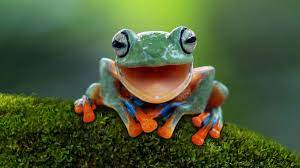
\includegraphics{download.jpeg}
    \caption{Example}
    \label{fig:results}
\end{figure}

Look at Figure~\ref{fig:results} for an example.

If~\cite{caselloTransportationActivityCenters2006} we want a page with no headers or footers except for a simple page number at the bottom we would use the keyword plain. However you need to be aware that using this command changes the page style for all the pages following the command. Therefore we need to turn the page style back to fancy as soon as we want the headers back.

If~\citep{caselloTransportationActivityCenters2006} we want a page with no headers or footers except for a simple page number at the bottom we would use the keyword plain. However you need to be aware that using this command changes the page style for all the pages following the command. Therefore we need to turn the page style back to fancy as soon as we want the headers back.

If~\citet{caselloTransportationActivityCenters2006} we want a page with no headers or footers except for a simple page number at the bottom we would use the keyword plain. However you need to be aware that using this command changes the page style for all the pages following the command. Therefore we need to turn the page style back to fancy as soon as we want the headers back.

This concludes our discussion on page layout. In the next post we'll look at using images and tables.If we want a page with no headers or footers except for a simple page number at the bottom we would use the keyword plain. However you need to be aware that using this command changes the page style for all the pages following the command. Therefore we need to turn the page style back to fancy as soon as we want the headers back.

This concludes our discussion on page layout. In the next post we'll look at using images and tables.If we want a page with no headers or footers except for a simple page number at the bottom we would use the keyword plain. However you need to be aware that using this command changes the page style for all the pages following the command. Therefore we need to turn the page style back to fancy as soon as we want the headers back.

This concludes our discussion on page layout. In the next post we'll look at using images and tables.If we want a page with no headers or footers except for a simple page number at the bottom we would use the keyword plain. However you need to be aware that using this command changes the page style for all the pages following the command. Therefore we need to turn the page style back to fancy as soon as we want the headers back.

This concludes our discussion on page layout. In the next post we'll look at using images and tables.If we want a page with no headers or footers except for a simple page number at the bottom we would use the keyword plain. However you need to be aware that using this command changes the page style for all the pages following the command. Therefore we need to turn the page style back to fancy as soon as we want the headers back.

This concludes our discussion on page layout. In the next post we'll look at using images and tables.If we want a page with no headers or footers except for a simple page number at the bottom we would use the keyword plain. However you need to be aware that using this command changes the page style for all the pages following the command. Therefore we need to turn the page style back to fancy as soon as we want the headers back.

This concludes our discussion on page layout. In the next post we'll look at using images and tables.If we want a page with no headers or footers except for a simple page number at the bottom we would use the keyword plain. However you need to be aware that using this command changes the page style for all the pages following the command. Therefore we need to turn the page style back to fancy as soon as we want the headers back.

This concludes our discussion on page layout. In the next post we'll look at using images and tables.If we want a page with no headers or footers except for a simple page number at the bottom we would use the keyword plain. However you need to be aware that using this command changes the page style for all the pages following the command. Therefore we need to turn the page style back to fancy as soon as we want the headers back.

This concludes our discussion on page layout. In the next post we'll look at using images and tables.If we want a page with no headers or footers except for a simple page number at the bottom we would use the keyword plain. However you need to be aware that using this command changes the page style for all the pages following the command. Therefore we need to turn the page style back to fancy as soon as we want the headers back.

This concludes our discussion on page layout. In the next post we'll look at using images and tables.If we want a page with no headers or footers except for a simple page number at the bottom we would use the keyword plain. However you need to be aware that using this command changes the page style for all the pages following the command. Therefore we need to turn the page style back to fancy as soon as we want the headers back.

This concludes our discussion on page layout. In the next post we'll look at using images and tables.If we want a page with no headers or footers except for a simple page number at the bottom we would use the keyword plain. However you need to be aware that using this command changes the page style for all the pages following the command. Therefore we need to turn the page style back to fancy as soon as we want the headers back.

This concludes our discussion on page layout. In the next post we'll look at using images and tables.If we want a page with no headers or footers except for a simple page number at the bottom we would use the keyword plain. However you need to be aware that using this command changes the page style for all the pages following the command. Therefore we need to turn the page style back to fancy as soon as we want the headers back.

This concludes our discussion on page layout. In the next post we'll look at using images and tables.If we want a page with no headers or footers except for a simple page number at the bottom we would use the keyword plain. However you need to be aware that using this command changes the page style for all the pages following the command. Therefore we need to turn the page style back to fancy as soon as we want the headers back.

This concludes our discussion on page layout. In the next post we'll look at using images and tables.If we want a page with no headers or footers except for a simple page number at the bottom we would use the keyword plain. However you need to be aware that using this command changes the page style for all the pages following the command. Therefore we need to turn the page style back to fancy as soon as we want the headers back.

This concludes our discussion on page layout. In the next post we'll look at using images and tables.If we want a page with no headers or footers except for a simple page number at the bottom we would use the keyword plain. However you need to be aware that using this command changes the page style for all the pages following the command. Therefore we need to turn the page style back to fancy as soon as we want the headers back.

This concludes our discussion on page layout. In the next post we'll look at using images and tables.If we want a page with no headers or footers except for a simple page number at the bottom we would use the keyword plain. However you need to be aware that using this command changes the page style for all the pages following the command. Therefore we need to turn the page style back to fancy as soon as we want the headers back.

This concludes our discussion on page layout. In the next post we'll look at using images and tables.

\chapter{Conclusion}
In conclusion, the methodology presented in this dissertation is a useful tool for transport planners to predict the trip attractiveness of a given area in Greater London based on its amenity and connectivity profile. By using SHAP values to extract local importance, we can identify destination hotspots based on the amenity profile of an area, which can be useful for local urban planners to identify areas that are popular for non-commute activities. However, the methodology is not without its limitations, and further work is needed to improve its generalisability and applicability in certain cases.

[to be completed]

\appendix
\chapter{Appendix}
\section{Open data sources}

The analysis carried out in this dissertation will utilise the Greater London area as the working case study, serving as an example for further replications of the analysis for other localities. The Office for National Statistics (ONS) defines the Greater London metropolitan area to include the City of London and the 32 London boroughs, with a total area of 1,572 km$^2$ and a population of 9.4 million people, making it the largest in the United Kingdom. The choice of the Greater London metropolitan area is also motivated by the availability of open data sources from which necessary features could be derived and the complexity of the public transport network that is coupled with rich usage data made available to the public. The data sources used in this analysis are summarised in Table \ref{tab:datasources} and detailed below.


\begin{table}[ht]
    \centering
    \renewcommand{\arraystretch}{1.5}
    \begin{tabular}{|l|l|l|}
        \hline 
        \rowcolor{lightgray}
        \textbf{} & \textbf{Variables} & \textbf{Sources} \\
        \hline

        \multirow{2}{12em}{\textbf{Public transport arrivals (target)}} 
        & Tube and Rail station exits & TfL network demand (NUMBAT) \\ 
        & Bus alightings & TfL network demand (BUSTO) \\
        \hline

        \textbf{Population} & Population count & UK Census 2021 \\
        \hline

        \multirow{2}{12em}{\textbf{Amenity Profile}} 
        & POI count by type & OSM Amenity POIs \\ 
        & POI diversity index & \\ 
        \hline 

        \multirow{3}{12em}{\textbf{Public Transport (PT) Connectivity Profile}} 
        & PT node count by type &  \\
        & PT node diversity index & OSM Transport POIs and TfL \\
        & PT network centrality &  \\
        \hline

            \end{tabular}
    \caption{Summary of data used in the analysis and their sources}
    \label{tab:datasources}
\end{table}

\subsubsection*{Transport for London (TfL) Open Data}

We use the following GIS datasets from the \href{https://gis-tfl.opendata.arcgis.com/}{TfL GIS Open Data Hub} and \href{https://api.tfl.gov.uk/}{TfL API} to derive transport-related features for the study area including density of transport facilities, diversity of transport options, and accessibility in the form of centrality measures in the Rail and Bus networks separately. The networks of interest are defined as follows:

\begin{itemize}
    \setlength\itemsep{0em}
    \item \textit{Rail network} includes the London Underground, London Overground, the Docklands Light Railway, and the Elizabeth Line, excluding stations and segments that are not managed by TfL or fall outside the Greater London area.
    \item \textit{Bus network} includes stop locations and route data of all bus and tram services, excluding stops and route segments that are not managed by TfL or within the Greater London area.
\end{itemize}

TfL also provides annually-updated \href{http://crowding.data.tfl.gov.uk/}{network demand datasets}, which will be used to derive the target variable of our analysis. The datasets are special interest to our analysis are namely \textit{Rail demand data (NUMBAT)} and the \textit{Bus demand data (BUSTO)}, from which we will extract estimated counts of station exits and bus alightings at the station or stop level, respectively. The dataset's temporal granularity is also an important aspect to consider. To address non-commute trips for the analysis, we will specifically use \textbf{Saturday average demand}, representing the demand in a typical period without any major citywide disruptions or events\footnote{This Saturday travel demand may still include work trips for those working on Saturdays, albeit not concentrated into peak periods as with weekday travel demand. For the scope of this analysis, we will treat these potential work trips as non-commute.}. To examine possible variations between different times of day, besides the total daily counts of exits and bus alightings, we will aggregate the data into four larger time bands\footnote{The choice of time band delineation is a compromise between different granularity levels afforded by the TfL rail and the bus demand datasets. There are opportunities to deepen the analysis by further segmenting the time bands into finer intervals if data permits.}:

\begin{itemize}
    \setlength\itemsep{-0.2em}
    \item \textit{Morning} (05:00 - 10:00): Limited mobility expected due to early hours
    \item \textit{Midday} (10:00 - 19:00): High daytime mobility expected
    \item \textit{Evening} (19:00 - 00:00): High evening mobility expected
    \item \textit{Late} (00:00 - 05:00): Minimal mobility expected due to sparser night PT services
\end{itemize}

It is worth noting that despite the existence of the Oyster Card integrated fare system, TfL does not provide origin-destination data for individuals as open data. Therefore, station exits and bus alightings are not directly associated with the number of passengers traversing through the system but are treated as discrete events. For example, a person who takes a bus to reach a Tube station for onward travel and then exits to arrive at their destination would be counted as two separate data points, one alighting for the bus and one station exit for the Tube. Nevertheless, our model will take this into account when making porediction and allows us to investigate patterns and the contribution of modal interchange behaviour in our interpretation.

Lastly, we need to acknowledge the particularity of the TfL bus demand dataset (BUSTO). Although passengers do not 'tap off' when alighting from busses, TfL has developed a methodology to estimate the number of passengers alighting at each bus stop based on individuals' next actions and other statistical methods. The methodology is described in detail in the \href{http://crowding.data.tfl.gov.uk/BUSTO/BUSTO\%20User\%20Guide\%20and\%20Data\%20Dictionary\%20v1.0.pdf}{BUSTO User Guide and Data Dictionary}

\subsubsection*{UK Census Data 2021}
For the estimated population datasets, we rely on the most recent United Kingdom Census data administered in 2021. The data is ingested at the Output Area (OA) level, which is the smallest geographical unit for which census data is available. Further processing will aggregate the data to the desired spatial unit of analysis.

\subsubsection*{OpenStreetMap POIs}
OpenStreetMap (OSM) is a collaborative mapping project that provides a free and open-source map of the world. The version of OSM data used in this analysis is packaged by an OpenStreetMap community project \href{https://www.geofabrik.de/en/geofabrik/openstreetmap.html}{Geofabrik} and provides a snapshot of the OSM database as of June 2024. Geofabrik also standardises the categorisation of POIs' amenity attributes in the OSM database into larger classes\footnote{More information about Geofabrik's OSM data product can be found in \href{https://www.geofabrik.de/data/geofabrik-osm-gis-standard-0.6.pdf}{Geofabrik OSM data dictionary}}. Our analysis will use this default POI classification, extracting 12 amenity POI types. Lastly, apart from amenity POIs, we also make use of the OSM transport POIs point data to derive non-TfL transport-related features, such as national rail stations, ferry piers, long-distance bus stations and airports. 

Combined with transport node data acquired from TfL open data sources, all extracted Amenity and Transport POI types of interest are summarised in Table \ref{tab:osmpoi}.

\begin{table}[ht]
    \centering
    \renewcommand{\arraystretch}{1.1}
    \begin{tabular}{|l|l|l|}
        \hline
        \rowcolor{lightgray}
        & \textbf{POI Type} & \textbf{Examples} \\
        \hline
        \multirow{13}{*}{\textbf{Amenity}}
            &\textit{Public Facilities} & Post offices, schools, universities, libraries,... \\
            &\textit{Medical} & Hospitals, clinics, pharmacies,... \\
            &\textit{Entertainment} & Theatres, Night clubs, cinemas,... \\
            &\textit{Outdoors} & Parks, playgrounds,... \\
            &\textit{Active} & Sports centres, swimming pools, stadiums,... \\
            &\textit{Restaurants} & Restaurants, cafes, pubs, bars,... \\
            &\textit{Hotels} & Hotels, motels, hostels,... \\
            &\textit{Shopping} & Supermarkets, bakeries, florists, bookshops, malls,... \\
            &\textit{Banking} & Banks, ATMs,... \\
            &\textit{Tourism} & Tourist attractions, museums, monuments, viewpoints,... \\
            &\textit{Religious} & Churches, mosques, temples,... \\
            &\textit{Nature} & Riverbanks, beaches, hills,... \\
        \hline
        \multirow{3}{*}{\textbf{Transport}}
            &\textit{Bus stops} & Bus stops and stations (TfL) \\
            &\textit{Rail stations} & TfL rail stations (TfL) and Non-TfL rail stations (OSM) \\
            &\textit{Other transport hubs} & Airports, ferry piers, long-distance bus stations (OSM) \\
        \hline
    \end{tabular}
    \caption{Summary of Amenity and Transport POI types used in the analysis}
    \label{tab:osmpoi}
\end{table}

\section{True to Data and True to Model in SHAP technique}

One ongoing debate regarding the use of SHAP for explainable is captured by \citet{chenTrueModelTrue2020}'s work exploring 'True to Model' versus 'True to Data' explanations. The 'True to Data' approach produces \textit{observational SHAP values} which reflect how a feature contributes to the model's prediction when considering the dependencies and correlations present in the training data, whereas the 'True to Model' approach produces \textit{interventional SHAP values} which reveal how a feature influences the model's prediction if we manipulate it independently, regardless of how it might interact with other features in reality. In our case, as we are more interested in observing feature contribution to the model prediction in a controlled environment rather than observing the relationships between features, we will use the 'True to Model' approach to interpret the model's prediction made possible by the \textit{shap} package.

\section{Supplemental Figures}
\begin{figure}[ht]
    \centering
    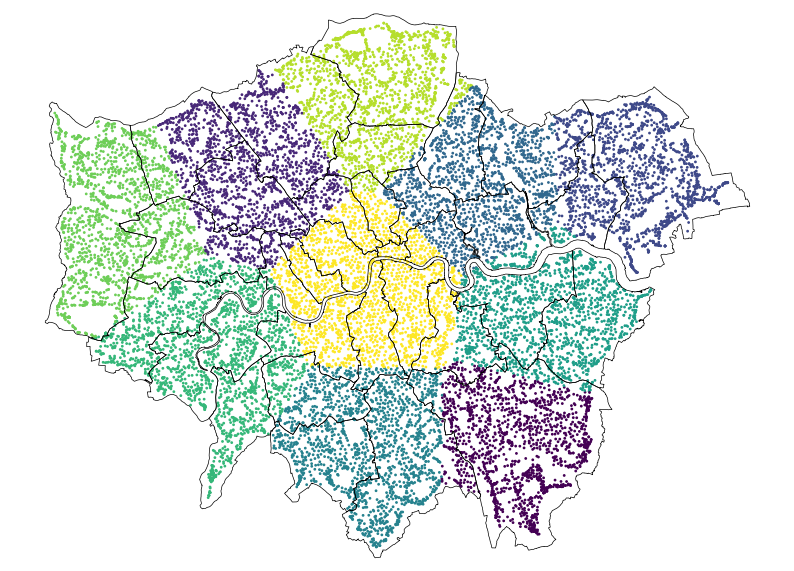
\includegraphics[width=0.5\textwidth]{kfold.png}
    \captionsetup{justification=centering}
    \caption{Map of the spatial k-fold cross-validation splits\\for hyperparameter tuning and performance assessment (k=10)}
    \label{fig:kfold}
\end{figure}

\begin{figure}[!ht]
    \centering
    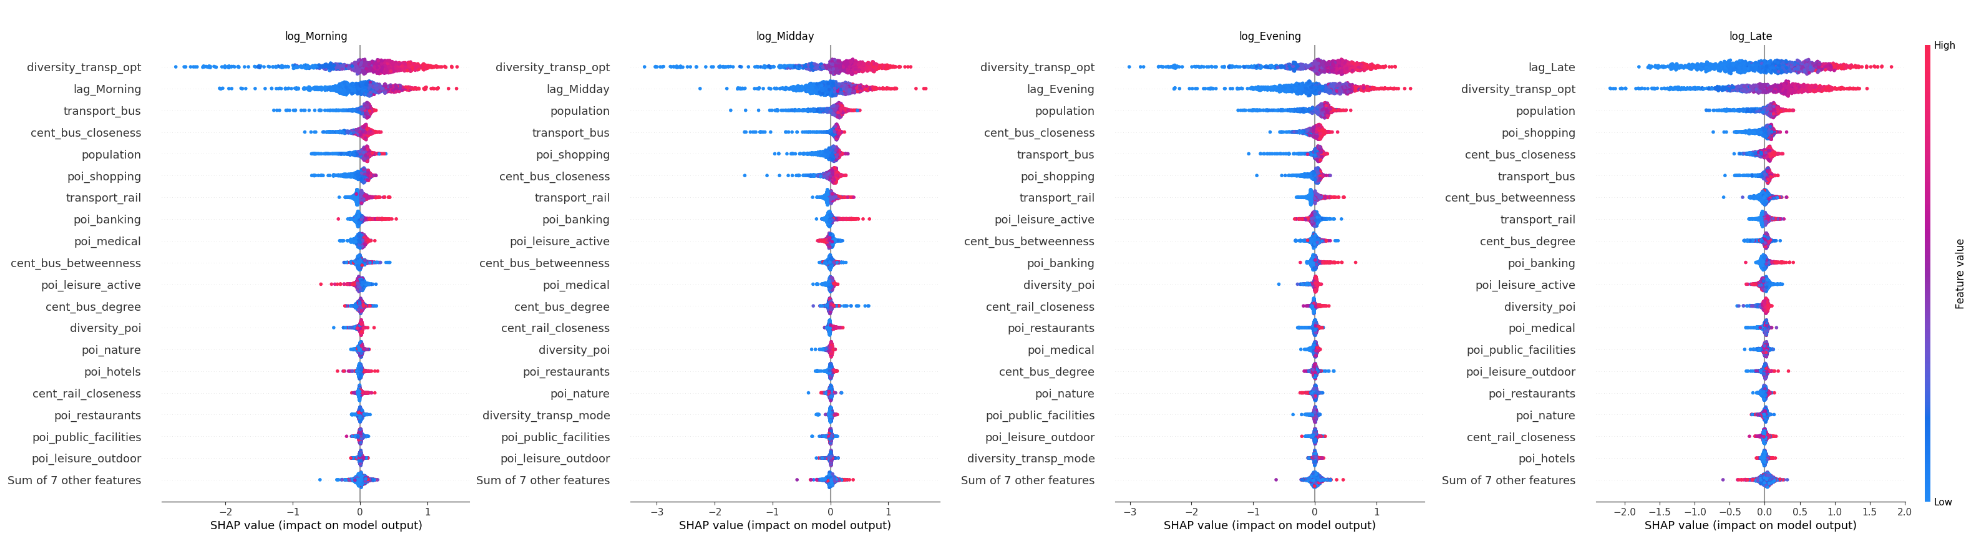
\includegraphics[width=\textwidth]{summarytimeband.png}
    \captionsetup{justification=centering}
    \caption{Summary of feature importance based on SHAP values of a sample. Red-Blue scale represents the feature value, and the x-axis represents the SHAP value, i.e., impact on final model prediction of arrivals in each time band (log)}
    \label{fig:beeswarmtimeband}
\end{figure}

\printbibliography{}

\end{document}